\documentclass{article}
\usepackage{amsthm}
\usepackage{amsmath}
\usepackage{graphicx}
\usepackage{tikz}
\usetikzlibrary{%
  arrows,%
  shapes.misc, 
  chains,%
  decorations.pathmorphing
}
\newtheorem{problem}{Problem}

\begin{document}
\title{Discrete Event Simulation}
\author{Henry Z. Lo}
\maketitle

\section{Motivation}
Suppose you were a branch manager of a bank.  How many tellers should you staff to keep customers happy?

With prior knowledge of how often customers come in, how fast it takes to serve a customer, and how long customers wait before leaving, it is possible to answer this question using a simulation:
\begin{itemize}
\item Start with $k$ tellers.
\item Customers enter the bank at rate $\lambda_1$.
\begin{itemize}
\item If a customer enters when a teller is free, process the customer.
\item Otherwise put customer in a queue.
\end{itemize}
\item Customers get processed at rate $\lambda_2$, after which the teller is freed and handles the next customer from the dequeue.
\end{itemize}

See Figure \ref{bank} for a diagram.  In this simulation, we can measure performance in terms such as average queue length, average wait time, etc.

\begin{figure}
\tikzset{
  nonterminal/.style={
    rectangle,
    very thick,
    font=\itshape
  },
  terminal/.style={
    rounded rectangle,
    very thick,
    font=\ttfamily}
}
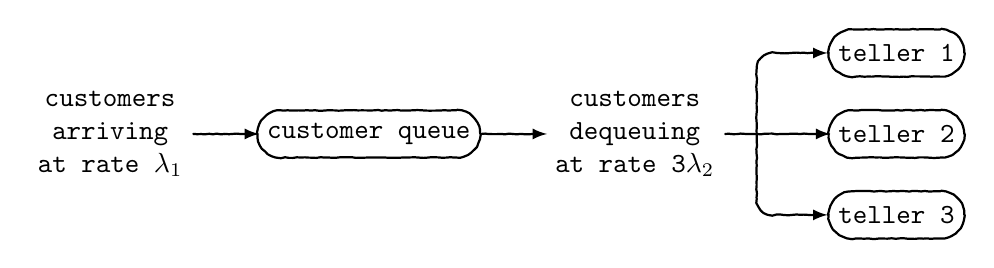
\begin{tikzpicture}[
    >=latex,thick,
    /pgf/every decoration/.style={/tikz/sharp corners},
    fuzzy/.style={decorate,
        decoration={random steps,segment length=0.5mm,amplitude=0.15pt}},
    minimum size=6mm,line join=round,line cap=round,
    terminal/.style={rectangle,draw,fill=white,fuzzy,rounded corners=3mm},
    nonterminal/.style={fill=white,fuzzy},
    node distance=4mm
  ]

    \ttfamily
    \begin{scope}[start chain,
            every node/.style={on chain},
            terminal/.append style={join=by {->,shorten >=-1pt,
                fuzzy,decoration={post length=4pt}}},
            nonterminal/.append style={join=by {->,shorten >=-1pt,
                fuzzy,decoration={post length=4pt}}},
            support/.style={coordinate,join=by fuzzy}
        ]
        \node [nonterminal, align=center] {customers \\arriving \\at rate $\lambda_1$};
        \node [support]                            {};
        \node [terminal]            (queue)        {customer queue};
        \node [support]                            {};
        \node [nonterminal, align=center] {customers \\dequeuing \\at rate 3$\lambda_2$};
        \node [support]             (after E)      {};
        \node [terminal,xshift=5mm]  (between)      {teller 2};
    \end{scope}
    \node (plus)  [terminal,above=of between] {teller 1};
    \node (minus) [terminal,below=of between] {teller 3};

    \begin{scope}[->,decoration={post length=4pt},rounded corners=2mm,
            every path/.style=fuzzy]
        \draw (after E)     |- (plus);
        \draw (after E)     |- (minus);
    \end{scope}
\end{tikzpicture}
\caption{Diagram demonstrating bank teller problem, with 3 tellers. \label{bank}}
\end{figure}

$\lambda_1$ and $\lambda_2$ can represent a probability distribution of values (e.g. Poisson) rather than a single rate, but both cases are handled similarly.

\section{Techniques}
In general, there are two methods of performing this type of simulation:
\begin{itemize}
\item Simulate the passage of time, then calculate what events happened in the time period.
\item Calculate when future events will happen (updating as needed), and then jump from event to event through time.
\end{itemize}

\subsection{Time-driven simulation}
Time-driven simulations often need a time jump interval $dt$ to be specified.  The general procedure:

\begin{enumerate}
\item Move forward $dt$ time units.
\item Calculate all events that happened within that time frame, and take them into account.
\item Loop back to 1 until complete.
\end{enumerate}
For our bank example:
\begin{enumerate}
\item Move forward $dt$ time units.
\item Process events in this time span:
\begin{itemize}
\item If there are customers being processed, subtract $dt$ from their process time; finish processing a customer if time exceeds $\lambda_2$.
\item Subtract $\lambda_1$ from the time until next customer, resetting the time and adding customers as necessary.
\item If a teller is free, dequeue a customer and start processing.
\end{itemize}
\item Loop back to 1 until complete.
\end{enumerate}

Note that calculating exactly what events occurred in the time step can be fairly difficult (which checks do we do first?).  Thus, typically they are synchronized to the end of each leap, i.e. events such as dequeuing and queuing only happen at the end of each time leap.

This can be simplified by a smaller $dt$, but this means we have to run many more checks.  It may make more sense to model event-by-event instead.

\subsection{Event-driven simulation}
Event-driven simulations can be more difficult to program, but are more accurate and faster.  The idea is:

\begin{enumerate}
\item Add an initial set of events to happen in the future.
\item Move to the first event to happen in this set.
\item Remove this event, and add new events spawned off by this event.
\item Repeat from step 2 until done.
\end{enumerate}

What data structure is optimal for storing events and when they occur?  Priority queues!  For our bank teller example:
\begin{enumerate}
\item Queue event "new customer" with time $1/\lambda_1$.
\item Dequeue soonest event from priority queue, and subtract that time from all event times.
\begin{itemize}
\item If event is "new customer" and
\begin{itemize}
\item if a teller $i$ is free, mark teller $i$ as occupied, then add event "customer done at teller $i$" in $1/\lambda_2$.
\item if no teller is free, put customer into customer queue. 
\end{itemize}
\item If event is "customer done at teller $i$" and
\begin{itemize}
\item if the customer queue is not empty, then dequeue a customer, mark teller $i$ as occupied, then add event "customer done at teller $i$" in $1/\lambda_2$.
\item if the customer queue is empty, then mark $i$ as free.
\end{itemize}
\end{itemize}
\item Repeat step 2 until done.
\end{enumerate}

As events are precomputed in the past, they do not need to be checked at every time step as in time-driven simulations.  This makes the simulation process much quicker.

If we want to see the changes between events, e.g. for visualization purposes, then we can run the simulation without having to check for events, until a scheduled event occurs.  We demonstrate this with another example.

\section{Particle Collisions}
Given a bunch of particles (assumed to be spheres), how can you simulate them bouncing off of each other?

Assume each point is a square of size $2s$, a starting position $x,y$, and a starting velocity $v_x, v_y$.  There are two types of events in this system: collisions between points, and collisions between a point and a wall.  Suppose for the sake of simplicity, when two points collide sideways, they reverse horizontal direction, and when they collide vertically, they reverse vertical direction.  There is no gravity or air resistance.

The procedure goes as follows:

\begin{enumerate}
\item Delete the soonest event, subtract its time from all events.
\item Disregard the event if one of the particles have been involved in a collision since the event has been added.
\item Process the event, and add others if needed.
\begin{itemize}
\item If two particles are colliding, update velocities of colliding particles (reverse horizontal direction if horizontal collision, etc.)
\item Calculate future collisions for the particles with new velocities.
\item Perform similar calculations for particles colliding with walls.
\end{itemize}
\end{enumerate}

\subsection{Collision detection}
The time-driven solution is to perform collision detection at each time step or frame.  If particles overlap, then there was a collision.

In order to avoid error, the simulation must be rewound to when the collision occurred and reran in order.  Alternatively, we can simply bounce the particles when we detect the collision (rather than when the collision actually happens), and accept the error that comes with this.

There is also the problem of the length of timestep $dt$, as before.  When $dt$ is too large, we may miss some collisions altogether (see Figure \ref{particle-miss}).  When $dt$ is too small, then we have to check collisions many times.  In either case, if we have $n$ particles, we need to do $O(n^2)$ checks every time step.

\begin{figure}
\centering
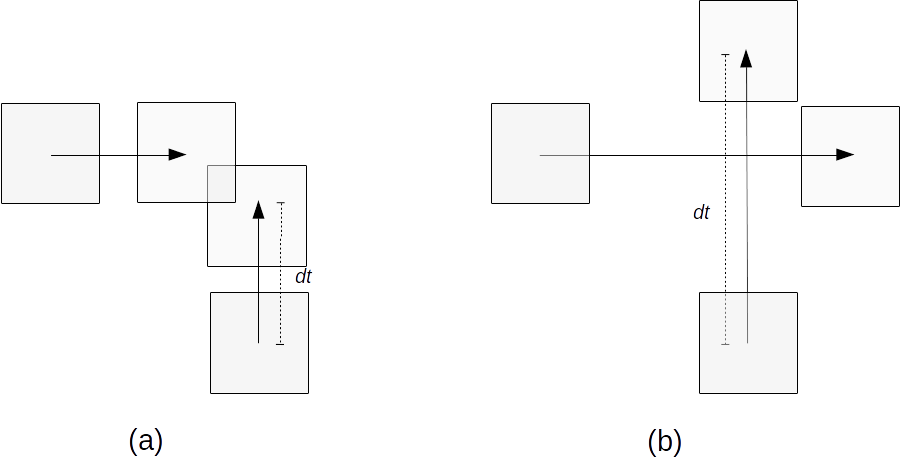
\includegraphics[scale=0.4]{img/particle-miss.png}
\caption{A collision between two particles (a) and two particles passing through each other due to a large $dt$ (b).  \label{particle-miss}}
\end{figure}


\subsection{Event-driven simulation}
At the beginning of the simulation, we first determine all the collisions that each particle will have - with the wall, and with each other.  As these collisions happen, we move through time and add more collisions to the priority queue, and invalidate some of the future reactions that were previously predicted to happen.

\subsubsection{Collisions with walls}
Collisions with walls are easiest to calculate, because the wall doesn't move.  

Suppose the walls exist at $x=0$, $y=0$, $x=1$, and $y=1$.  Then the time until the particle's edge collides with a wall is $t$, where:

\begin{align*}
x+s+v_xt=1 & \text{ if } v_x > 0 \\
x-s+v_xt=0 & \text{ if } v_x < 0 \\
y+s+v_yt=1 & \text{ if } v_y > 0 \\
y-s+v_yt=0 & \text{ if } v_y < 0 
\end{align*}

Collisions in $x$ don't affect collisions in $y$.  Solving for $t$:

\[t=
\begin{cases}
\frac{1-x-s}{v_x} & \text{if } v_x > 0 \\
\frac{-x-s}{v_x} & \text{if } v_x < 0 \\
\frac{1-y-s}{v_y} & \text{if } v_y > 0 \\
\frac{-y-s}{v_y} & \text{if } v_y < 0 
\end{cases}
\]

See Figure \ref{particle-wall} for a visual.

\begin{figure}
\centering
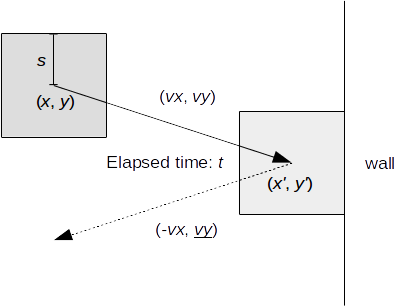
\includegraphics[scale=0.75]{img/particle-wall.png}
\caption{Collision of a particle with wall.  \label{particle-wall}}
\end{figure}

\subsection{Collisions between particles}
To simplify computations, let $s$ be the same for every particle.  There are two ways in which particles can collide - horizontally, after which they reverse horizontal directions, and vertically, in which case they reverse vertical directions.

Since $s$ is the same, one of the corners of one square must touch the edge of the other square.  In other words, we have a horizontal collision at time $t$:

\begin{itemize}
\item if $v_x > 0$, $x+s+v_xt = x'-s+v_x't$ (there is horizontal overlap) AND
\begin{itemize}
\item $y+s+v_yt$ is between $y'+s+v_y't$ and $y'-s+v_y't$ OR
\item $y-s+v_yt$ is between $y'+s+v_y't$ and $y'-s+v_y't$
\end{itemize}
\item if $v_x < 0$, $x-s+v_xt = x'+s+v_x't$ AND
\begin{itemize}
\item $y+s+v_yt$ is between $y'+s+v_y't$ and $y'-s+v_y't$ OR
\item $y-s+v_yt$ is between $y'+s+v_y't$ and $y'-s+v_y't$
\end{itemize}
\end{itemize}

The first case describes the first square going right, and the second square going left; the second case describes the opposite situation.  Similar equations need to be defined for vertical collisions.

We can solve either of these equations for the time of collision $t$:
\begin{align*}
x+s+v_xt &= x'-s+v_x't \\
x-x'+s+s &= v_x't -v_xt \\
\frac{x-x'+2s}{v_x'-v_x} &= t \\
\end{align*}

\end{document}
